

%----------------------------------------------------------------------------------------
%	PACKAGES AND DOCUMENT CONFIGURATIONS
%----------------------------------------------------------------------------------------

\documentclass[a4paper,12pt]{article}
\usepackage{siunitx} % Provides the \SI{}{} and \si{} command for typesetting SI units
\usepackage{graphicx} % Required for the inclusion of images
\usepackage{subfigure}
\usepackage{multirow}
\usepackage{amsmath} % Required for some math elements 
\usepackage{indentfirst}
\usepackage{times} % Uncomment to use the Times New Roman font
\usepackage{appendix}
\usepackage{verbatim}

%----------------------------------------------------------------------------------------
%	DOCUMENT INFORMATION
%----------------------------------------------------------------------------------------

\title{ \rule{\textwidth}{0.3mm} \\UM–SJTU JOINT INSTITUTE \\ PHYSICS LABORATORY \\ (VP141) \\ \rule{\textwidth}{0.3mm} \\ [20 mm]  \Large{Laboratory Report} \\[5 mm]  Exercise 5 \\[1 mm] 
Damped and Driven Oscillations. \\Mechanical Resonance\\[20 mm]} % Title
\author{Cao Zhiyuan} % Author name
\date{\today} % Date for the report

\begin{document}
\scshape

\maketitle % Insert the title, author and date

\begin{center}
\begin{tabular}{l l l}
\\[5 mm]
Partners:  \\
Name: Cao Zhiyuan & ID: 518370910030 & Group: 14 \\
Name: Jin Haoxiang & ID: 518370910215 & Group: 3 \\
~\\
Date Performed:\\
June 28, 2019\\
\end{tabular}
\end{center}

\thispagestyle{empty}


\newpage


\small\tableofcontents
\thispagestyle{empty}


\newpage

%----------------------------------------------------------------------------------------
%	SECTION 1
%----------------------------------------------------------------------------------------
\setcounter{page}{1}
\upshape
\section{\textsc{Introduction}}
In our daily life, oscillation occurs everywhere. From the resonator of the string instruments, to the construction of hyperelastic membrane are both examples of oscillation in our world. To further study the problem, we assume that a force changing periodically with time is applied to a damped harmonic oscillator, i.e. 
\begin{center}
$F_{dr} = F_0 cos \omega t$
\end{center}
where $F_{dr}$ is the external force called driving force, $F_0$ is the amplitude and $\omega$ is its angular frequency. After a period of time the motion will tend to be in equilibrium. The steady state is a simple harmonic oscillation with an angular frequency equal to that of the driving force. The amplitude depends on the driving force as well as the damping coefficient. In brief, such phenomenon is often called mechanical resonance. \par
Interestingly, after the oscillation reaches its equilibrium state, there will be a phase lag between the displacement from equilibrium position and the driving force. Particularly, the value equals to $\frac{\pi}{2}$ when the frequency of driving force is equal to the natural frequency. \par 
In our experiment, we will focus on forced oscillation of a balance wheel. Electromagnets provide us with a damping force. Since in our experiment, our system is rotating, the quantities are all expressed in terms of angular value. For example, the amplitude is expressed in terms of its angular equivalent.\par 
Then, we try to find out its numerical value. Assume that the wheel is exposed to a period driving torque $\tau_{dr} = \tau_0 cos\omega t$ and a damping torque $\tau_d = -b\frac{d\theta}{dt}$, with a restoring torque $\tau = -k\theta$. After that, we can write the equation of motion of the system:
\begin{equation}
I\frac{d^2\theta}{dt^2} = -k\theta -b\frac{d\theta}{dt} + \tau_0 cos\omega t
\end{equation}
where $I$ refers to the moment of inertia, and $\tau_0$ as well as $\omega$ are the amplitude and frequency of $\tau_{dr}$ respectively. Then, we change its form, Eq.(1) turns out to be: 
\begin{center}
$\displaystyle \frac{d^2\theta}{dt^2} +\frac{b}{I}\frac{d\theta}{dt} + \frac{k}{I}\theta = \frac{\tau_0}{I} cos(\omega t)$
\end{center}
To further simplify its form, we replace some of parameters with the following symbols:
\begin{center}
$\displaystyle\omega_0^2 = \frac{k}{I}, ~ 2\beta = \frac{b}{I}, ~\mu = \frac{\tau_0}{I}$
\end{center}
Then, Eq.(1) can be expressed as:
\begin{equation}
\displaystyle \frac{d^2\theta}{dt^2} + 2\beta \frac{d\theta}{dt} + \omega_0^2 \theta = \mu cos(\omega t)
\end{equation}
\par Now, Eq(2) is an inhomogeneous ODE. We first consider the simplest case when $\mu = 0$. Then, it's an equation of motion for a damped harmonic oscillator. For a damped harmonic oscillator, the following possibilities exist: underdamped regime, overdamped regime and critical damping, and each of them has different $x-t$ curves. Furthermore, if in this case additionally $\beta = 0$ always holds, then the motion becomes a simple harmonic oscillation.
\par However, if $\mu \not = 0$, it's a little bit complicated. We solve the equation by first assuming the solution has the form:
\begin{center}
$\displaystyle \widetilde\theta(t) = A e^{i(\omega_{dr} t + \varphi)}$
\end{center}
Then, we obtain 
\begin{center}
$\displaystyle \dot{\widetilde{\theta(t)}} = iA\omega_{dr} e^{i(\omega_{dr} t + \varphi)} = i\omega_{dr}\widetilde\theta(t)$\\
[3 mm]
$\displaystyle \ddot{\widetilde{\theta(t)}} = -A\omega_{dr}^2 e^{i(\omega_{dr} t + \varphi)} = -\omega_{dr}^2\widetilde\theta(t)$
\end{center}
Plug them in Eq.(2), and we will obtain 
\begin{equation}
[(\omega_0^2-\omega_{dr}^2) + 2i\beta \omega_{dr}] A e^{i(\omega_{dr} t + \varphi)} = \mu cos\omega t
\end{equation}
Since we have
\begin{center}
$e^{i(\omega t + \varphi)} = cos(\omega t + \varphi) + i sin(\omega t + \varphi)$
\end{center}
we further obtain that 
\begin{center}
$Re~e^{i(\omega t + \varphi)} = cos(\omega t + \varphi) $
\end{center}
Plug it back to Eq.(3), and because $\omega_{dr} = \omega$, we have 
\begin{equation}
[(\omega_0^2-\omega^2) + 2i\beta \omega] A e^{i\varphi} = \mu
\end{equation}
For $(\omega_0^2-\omega^2) + 2i\beta \omega$ from the left hand side, we transform it into polar coordinates, and we will obtain:
\begin{center}
 $(\omega_0^2-\omega^2) + 2i\beta \omega = \sqrt{(\omega_0^2 - \omega^2) + 4\beta^2\omega^2}~e^{i\varphi'}$
\end{center}
where $\varphi' = arctan(\frac{2\beta \omega}{\omega_0^2-\omega^2})$. Then, we plug it in Eq.(4), and we acquire immediately 
\begin{equation}
\sqrt{(\omega_0^2 - \omega^2) + 4\beta^2\omega^2} A e^{i\varphi'} e^{i\varphi}= \mu
\end{equation}
In order that Eq.(5) holds, $\varphi' = - \varphi$. Hence, we finally obtain the value of $A$ and $\varphi$:
\begin{center}
$\left\{
\begin{aligned}
A = \frac{\mu}{\sqrt{(\omega_0^2 - \omega^2)^2 + 4\beta^2\omega^2}}
\\
\varphi = arctan(\frac{2\beta \omega}{\omega^2-\omega_0^2})~~~~~~~~
\end{aligned}
\right.$
\end{center}
\newpage
Therefore, we are able to calculate the solution to Eq.(2) in a general form, i.e.
\begin{equation}
\theta(t) = \theta_{tr}(t) + \theta_{st}cos(\omega t + \varphi)
\end{equation}
where $\theta_{tr}$ refers to the transient state which vanishes exponentially with the increase of t, and $\theta_{st}cos(\omega t + \varphi)$ refers to the steady-state situation, with an amplitude of the value:
\begin{center}
$\displaystyle \theta_{st} = \frac{\mu}{\sqrt{(\omega_0^2 - \omega^2)^2 + 4\beta^2\omega^2}} $
\end{center}
and the phase shift 
\begin{center}
$\displaystyle \varphi = arctan(\frac{2\beta \omega}{\omega^2-\omega_0^2})$
\end{center}
\par If we want to find out the maximum value of $\theta_{st}$, we can obtain the resonance angular frequency and its amplitude as follows:
\begin{center}
$\displaystyle \omega_{max} = \omega_{res} = \sqrt{\omega_0^2 - 2\beta^2}$\\[3 mm]
$\displaystyle \theta_{max} = \theta_{res} = \frac{\mu}{2\beta \sqrt{\omega_0^2 - \beta^2}}$
\end{center}
\par Specifically, if the damping coefficient is small, then the resonance angular frequency has a close value to the natural one. In Figure 2, the dependence of amplitude and phase shift on driving frequency are shown respectively \cite{labmanual}.
\begin{figure}[h] 
    \centering
    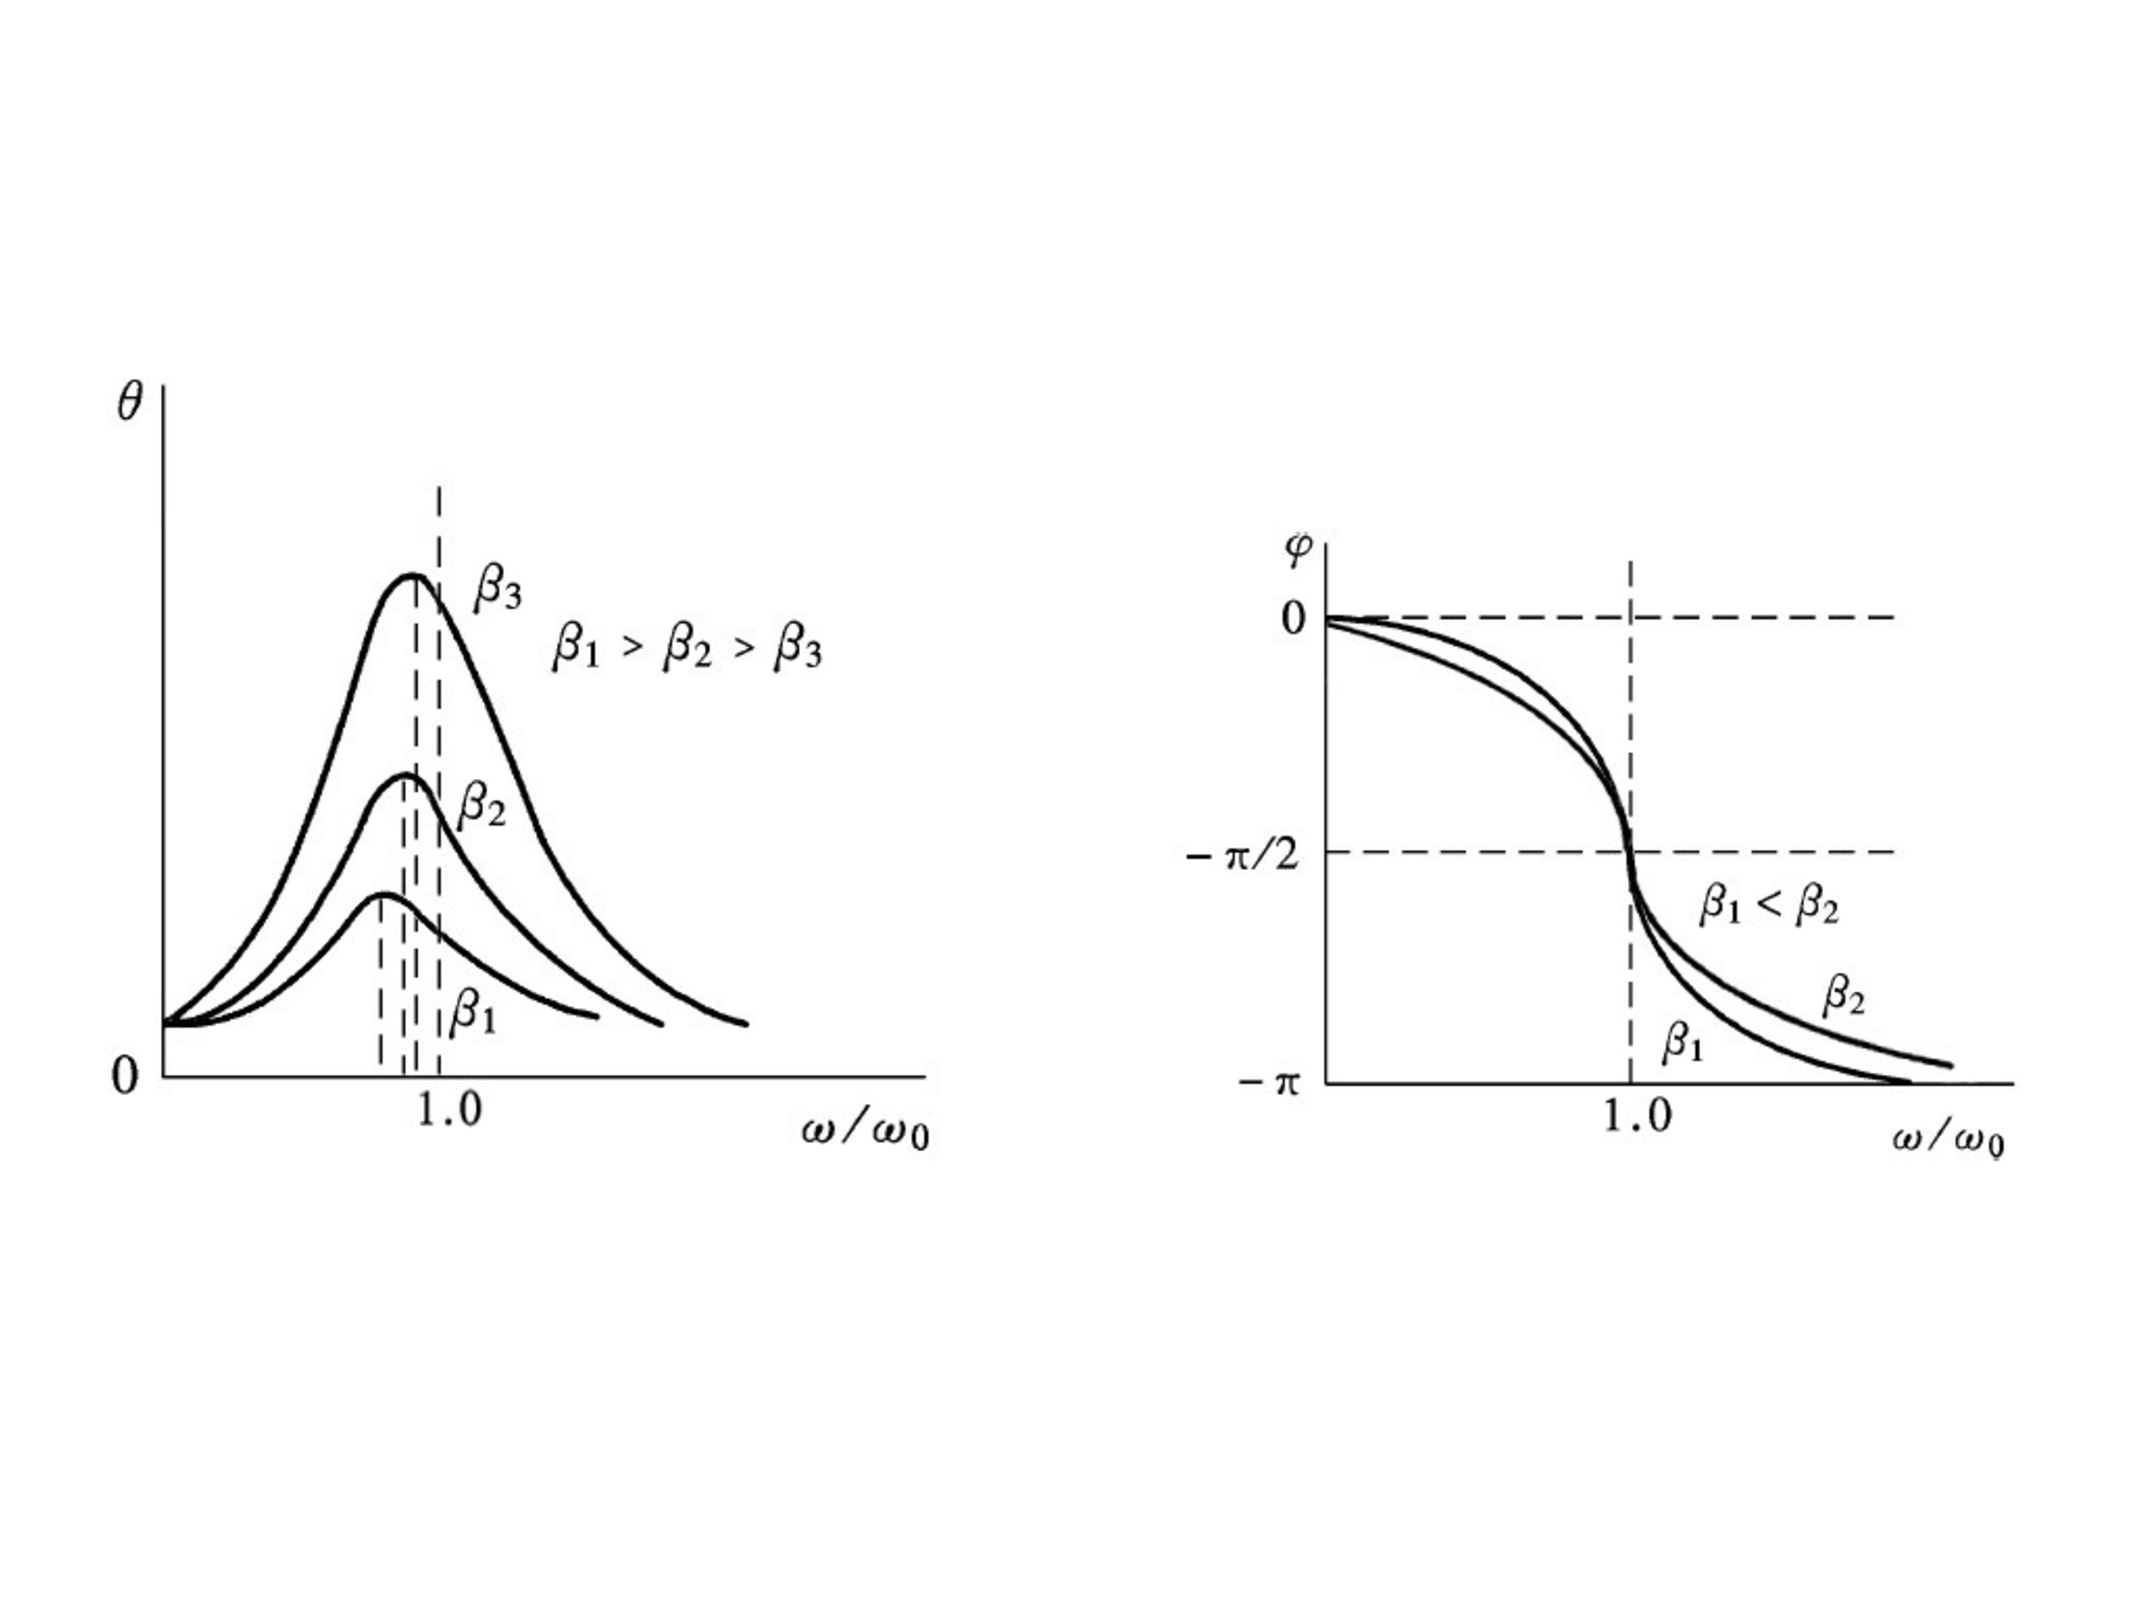
\includegraphics[width=1\textwidth]{Fig1} 
    \caption{The dependence of amplitude and phase shift on driving frequency \cite{labmanual}} 
\end{figure}

%----------------------------------------------------------------------------------------
%	SECTION 2
%----------------------------------------------------------------------------------------
\section{\textsc{Apparatus and Experimental Setup}}
The main apparatus we use in experiment is the BG-2 Pohl resonator, which is shown in Figure 1. BG-2 Pohl Resonator consists of two parts: a vibrometer and a control box.
\par 
The most noticeable part of the resonator is its balance wheel. The wheel is placed on a supporting nod, with its axis attached to a scroll spring, providing the wheel with restoring force to make it rotate periodically around its equilibrium position.
\par
The edge of the balance wheel consists of many grooves. A deep notch with a photodetector is arranged above one of them. The detector can be used to detect amplitudes and oscillation periods.
\par 
To equip the apparatus with the capability to create damping force, a pair of coils is placed at the bottom of the wheel. Due to some complicated electromagnetic actions, a damping force will be created so that we can simulate the cases of forced oscillations. 

\begin{figure}[h] 
    \centering
    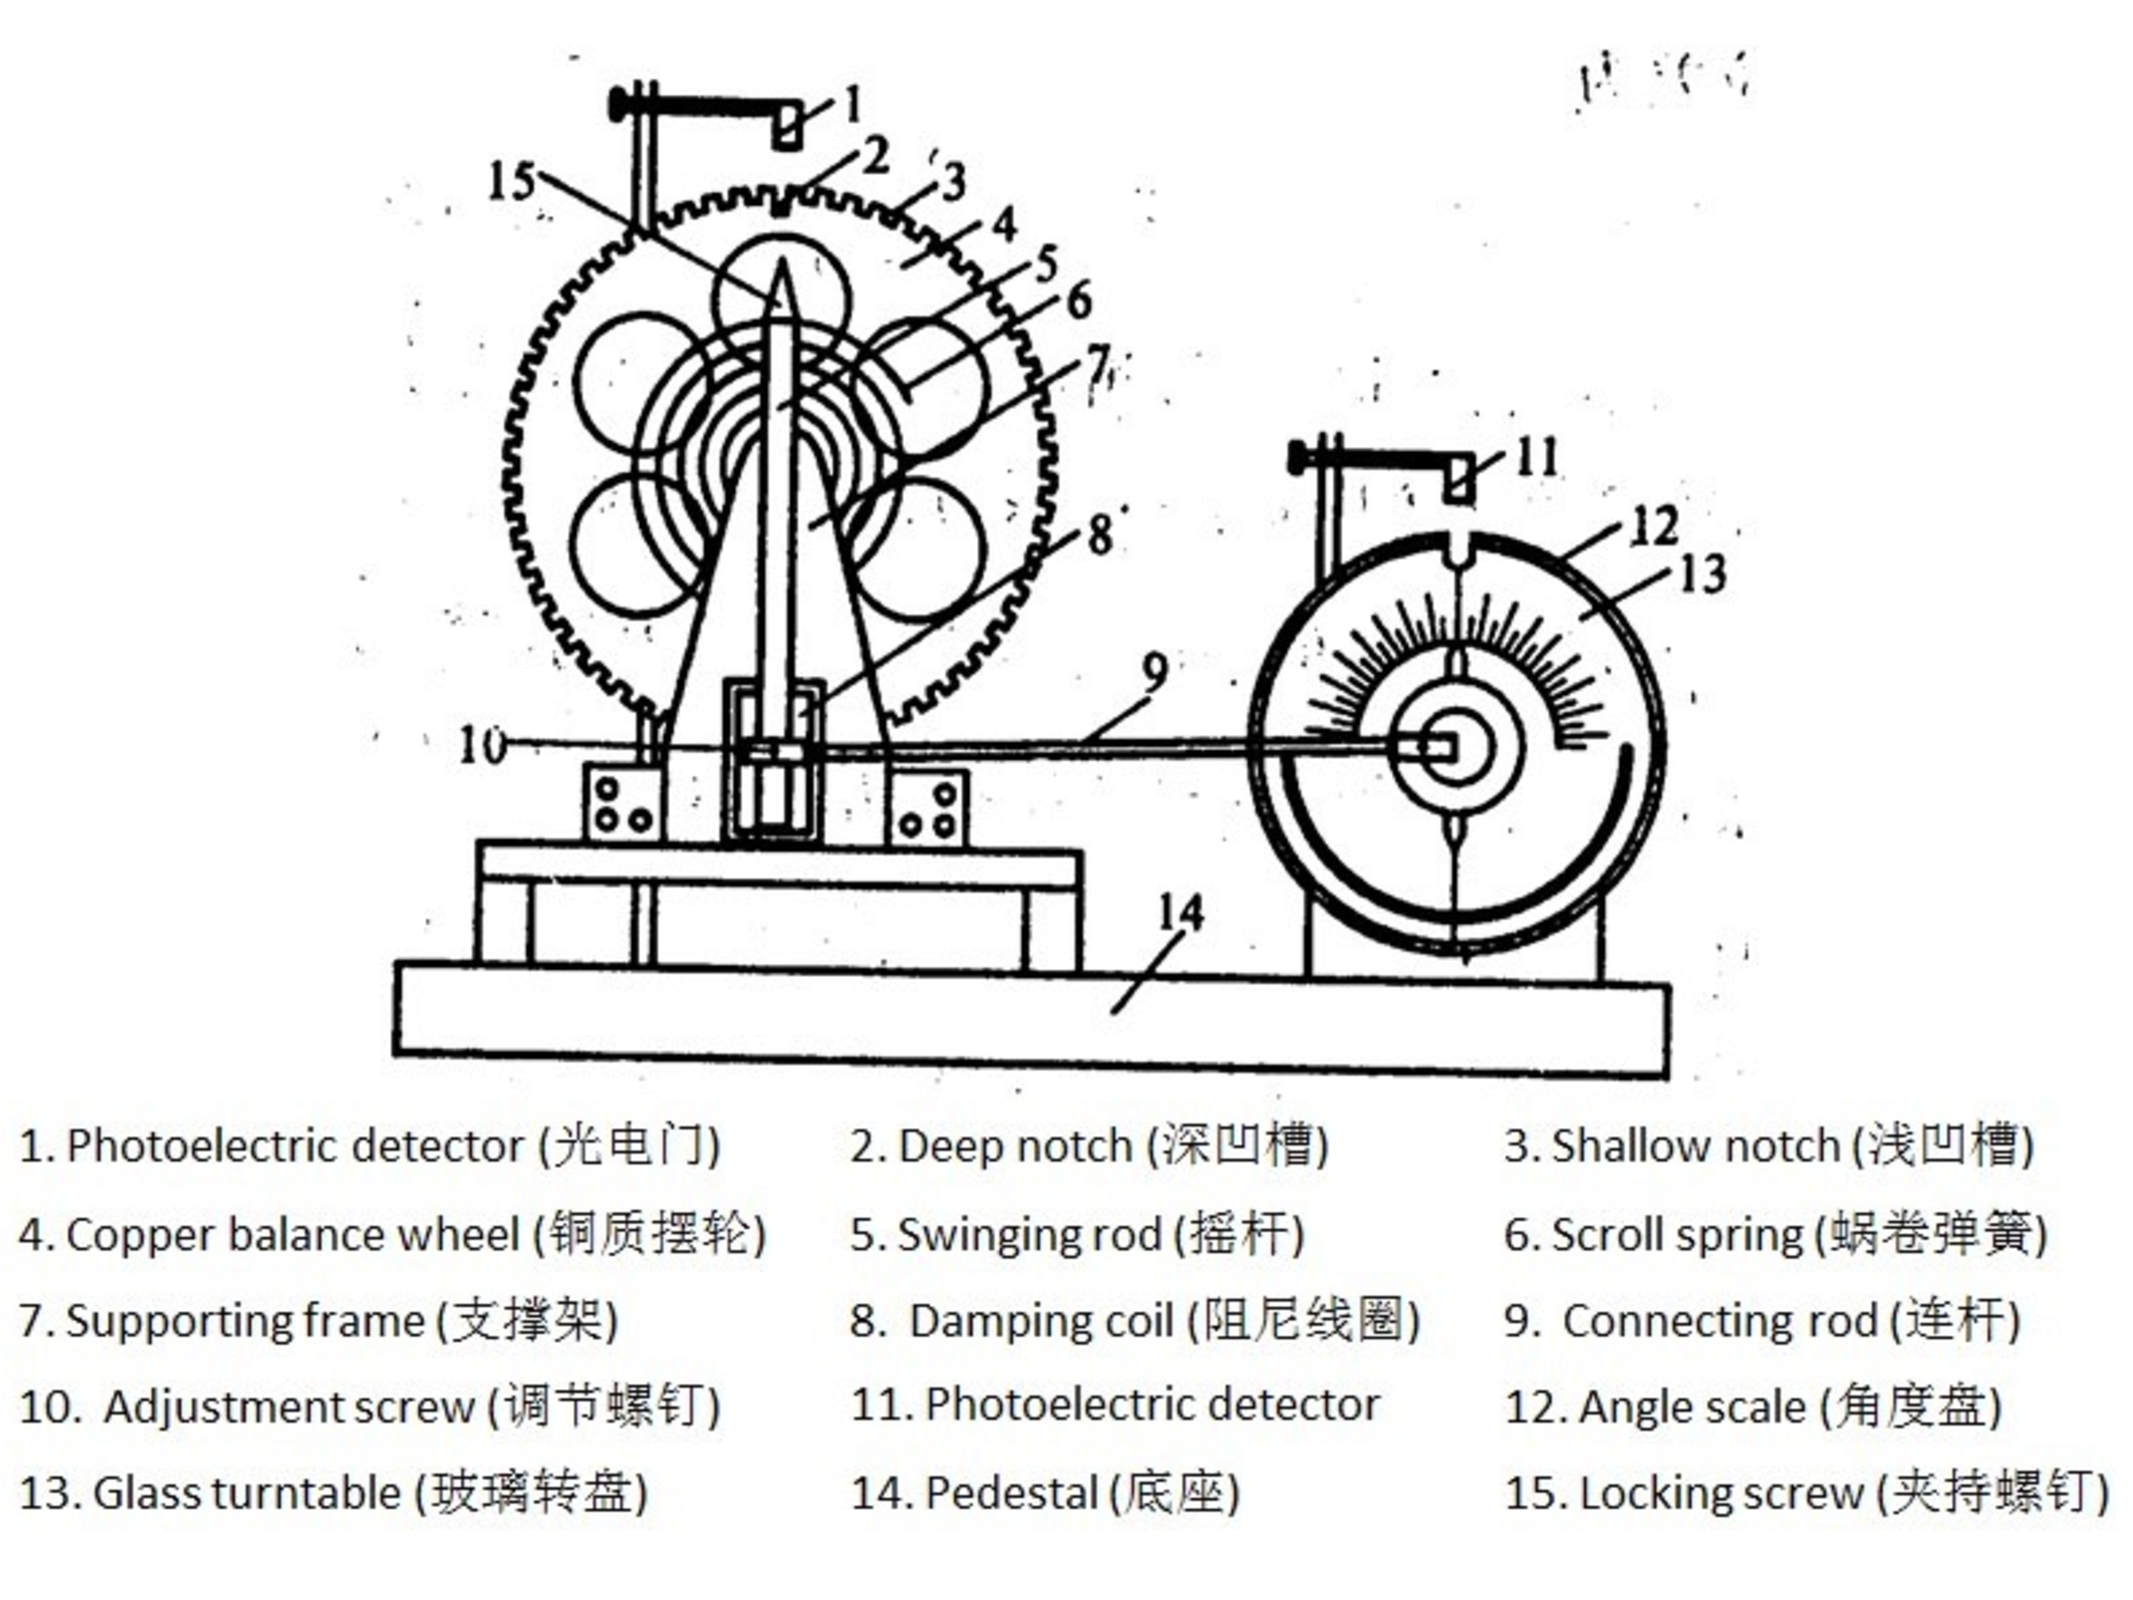
\includegraphics[width=1\textwidth]{Fig2} 
    \caption{The BG-2 Pohl resonator \cite{labmanual}} 
\end{figure}

\par 
As for how to use the resonator, there are a few knobs on it. For \textbf{Period Selection} switch, we can choose how to measure the period: 1-period mode and 10-period mode. For \textbf{Period of Driving Force} knob, the frequency and amplitude of the driving force can be changed accurately. However, the particular scale on it is inaccurate. Thus only the trend is controllable in our experiment.
\par 
In terms of \textbf{Damping Selection} nob, there are six options, i.e. "0", "1", "2", "3", "4", "5", "6" respectively. The current increase from 0 to 0.6 $A$ with the increase of option numbers. In this experiment, option "2", "3", "4" are used as damping mode.
\par 
There is also a \textbf{Strobe} bottom on our resonator. By turning on this bottom a flash light will be emitted so that we are able to read out the phase difference. However, in order to protect the strobe, only when measuring the phase difference will we turn on the bottom.
\par 
Also, there is a \textbf{Motor Switch} bottom which is used to control motor. When measuring natural angular frequency and damping coefficient, the bottom ought to be turned off. 
\par 
For the detail position of these bottoms, see the following Figure 3.

\begin{figure}[h] 
    \centering
    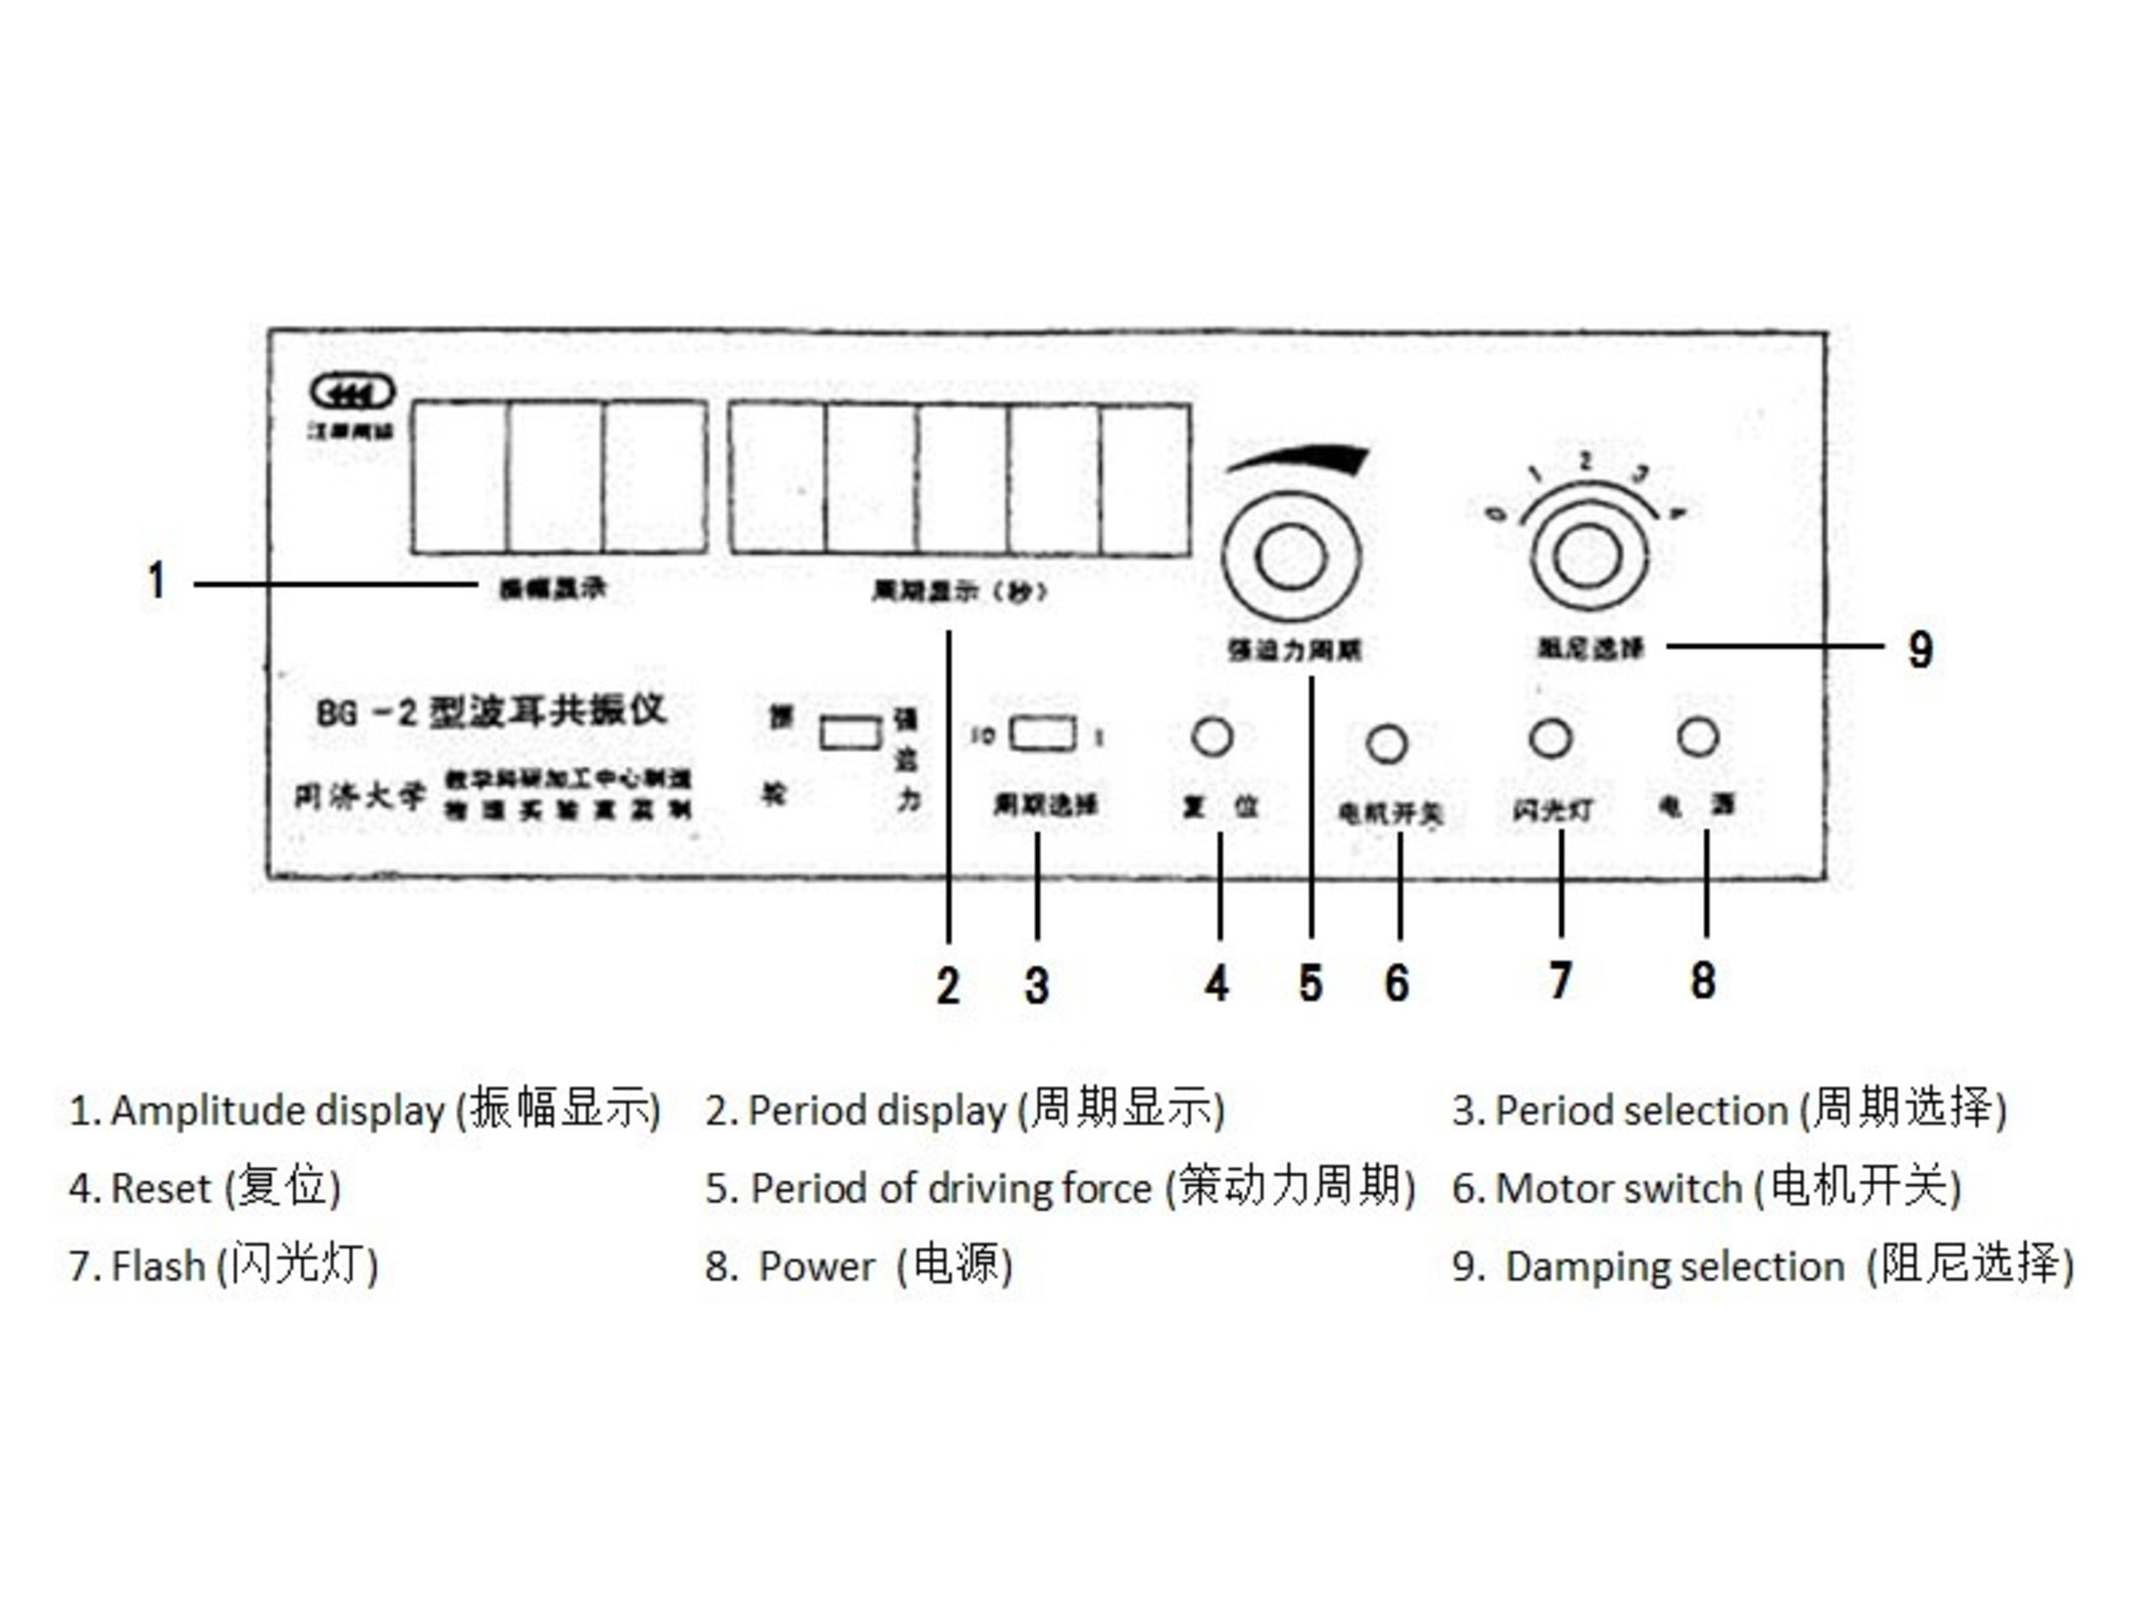
\includegraphics[width=1\textwidth]{Fig3} 
    \caption{The panel of control box \cite{labmanual}} 
\end{figure}

%----------------------------------------------------------------------------------------
%	SECTION 3
%----------------------------------------------------------------------------------------
\section{\textsc{Measurements}}
\subsection{\textsc{Procedures \cite{labmanual}}}
\subsubsection{\textsc{Natural Angular Frequency}}
\begin{itemize}
\item[(1)] Switch the \textbf{Damping Selection} bottom to "0".
\item[(2)] Rotate the balance wheel to approximately $150^{\circ}$ and then release it. Select the \textbf{Period Selection} switch to "10", record the period.
\item[(3)] Repeat four times and then obtain the natural angular frequency.
\end{itemize}
\subsubsection{\textsc{Damping coefficient}}
\begin{itemize}
\item[(1)] Switch the \textbf{Damping Selection} bottom to "2".
\item[(2)] Rotate the balance wheel to approximately $150^{\circ}$ and then release it. Record each amplitude (omit the first one) and the corresponding 10-periods.
\item[(3)] Calculate the damping coefficient through the following format:
\begin{center}
$\displaystyle ln\frac{\theta_i}{\theta_j} = (j-i) \beta t$
\end{center}
\item[(4)] In our experiment, calculate $T$ as the average period, then plug it in the equation:
\begin{center}
$\displaystyle \beta = \frac{1}{5T}ln\frac{\theta_i}{\theta_{i+5}}$
\end{center}
\end{itemize}
\subsubsection{The $\theta_{st}-\omega$ \textsc{and} $\varphi-\omega~$\textsc{Characteristics of Forced Oscillations}}
\begin{itemize}
\item[(1)] Switch the \textbf{Damping Selection} bottom to "2". Set the speed of motor to one end, and after it reaches the steady state, record the amplitude $\theta_{st}$, the period $T$, and the phase shift $\varphi$.
\item[(2)] Change the speed of motor slowly, then record the previous three values when it become steady. Collect at least 15 data points.
\item[(3)] Switch the \textbf{Damping Selection} bottom to "1" or "3" and repeat step (1) and (2).
\item[(4)] Plot $\displaystyle \theta_{st}(\omega) - \omega/\omega_0$ and $\displaystyle \varphi(\omega) - \omega/\omega_0$ characteristics respectively.
\end{itemize}
\subsection{\textsc{comments/observations regarding the measurements}}
In this experiment, there are some tips that we should take care of:
\begin{itemize}
\item[(1)] When calculating the natural angular frequency in Procedure 3.1.1, be careful with its uncertainty.
\item[(2)] In Procedure 3.1.2, omit the first amplitude before released because it may have a large deviation.
\item[(3)] In Procedure 3.1.2, if some data is missed in the step (2), the whole step should be done again.
\item[(4)] In Procedure 3.1.3, remember to wait a few seconds so that you determine the wheel has already been in steady state. Otherwise there may be some errors take place.
\end{itemize}
%----------------------------------------------------------------------------------------
%	SECTION 4
%----------------------------------------------------------------------------------------
\newpage 
\section{\textsc{Results}}
\subsection{\textsc{Natural Angular Frequency}}
The natural angular frequency was measured by releasing the balance wheel from 150 $^{\circ}$ and the corresponding 10 periods have been recorded in table 1 as
\begin{table}[h]
\begin{center}
\begin{tabular}{|c|c|}
\hline
   & $10T [s] \pm 0.001 [s]$ \\
\hline
1 & 15.812 \\
2 & 15.810 \\
3 & 15.810 \\
4 & 15.811 \\
\hline
\end{tabular}
\caption{Data table for Natural Angular Frequency}
\end{center}
\end{table}

Hence, we obtain the average period of the oscillator as follows:
\begin{center}
$\displaystyle \overline{10T} = \frac{1}{4}\sum_{i=1}^4 10T_i = 15.811 [s] \pm 0.002 [s]$ \\[3 mm]
$\displaystyle \overline{T} = \frac{\overline{10T}}{10} = 1.5811 [s] \pm 0.0002 [s]$
\end{center} 
with a relative uncertainty $\displaystyle u_T = 0.01 \%$.\\
\par 
Eventually, we can calculate the natural angular frequency 
\begin{center}
$\displaystyle \omega_0 = \frac{2\pi}{T} = 3.9739 [s^{-1}] \pm 0.0004[s^{-1}]$
\end{center}
with a relative uncertainty $\displaystyle u_{\omega_0} = 0.01 \%$. (The detailed calculations are shown in the Worksheet). 

\subsection{\textsc{Damping Coefficient}}
According to our measurements, our data is collected in Table 2.
From the reading on the control box, our damping selection and period of damping are shown as follows:

\begin{center}
Damping Selection: 2 \\[3 mm]
$\displaystyle T = \frac{10T}{T} = 1.5852 [s] \pm 0.0001 [s] $
\end{center}

According to the formula we deduced in 3.1.2, we can calculate the damping coefficient accordingly.
\begin{center}
$\displaystyle \beta = \frac{1}{5T}ln\frac{\theta_i}{\theta_{i+5}} = 0.056 [s^{-1}] \pm 0.004[s^{-1}]$
\end{center}
with a relative uncertainty $\displaystyle u_{\beta} = 7 \%$. (The detailed calculations are shown in the Worksheet). 

\begin{table}[h]
\begin{center}
\begin{tabular}{|c|c|c|c|c|}
\hline
\multicolumn{5}{|c|}{$10T = 15.852 [s] \pm 0.001 [s]$ \& Damping Selection: 2} \\
\hline
\multicolumn{2}{|c|}{Amplitude$[^\circ] \pm 1[^\circ]$} & \multicolumn{2}{c|}{Amplitude$[^\circ] \pm 1[^\circ]$} & ln$(\theta_i/\theta_{i+5})$\\
\hline
~$\theta_0$~ & 116 & ~$\theta_5$~ & 73 & 0.4631 \\
~$\theta_1$~ & 105 & ~$\theta_6$~ & 67 & 0.4493\\
~$\theta_2$~ & 96 & ~$\theta_7$~ & 62 & 0.4372\\
~$\theta_3$~ & 87 & ~$\theta_8$~ & 56 & 0.4406\\
~$\theta_4$~ & 79 & ~$\theta_9$~ & 51 & 0.4376\\
\hline
\multicolumn{4}{|c|}{The average value of ln($\theta_i/\theta_{i+5}$)} & 0.4456 \\
\hline
\end{tabular}
\caption{Data table for Resonance Method}
\end{center}
\end{table}
\subsection{The $\theta_{st}-\omega$ \textsc{and} $\varphi-\omega~$\textsc{Characteristics of Forced Oscillations}}
In this part, we use two different damping coefficients to measure the corresponding $\theta_{st}-\omega$ and $\varphi-\omega$ characteristics and then compare the following properties: the characteristics of the relationship between amplitude/phase lag and driving frequency, and their trends when changing the damping coefficients. We do two experiments choosing damping selection "2" and "3" respectively, and then record the data as follows (Table 3 and Table 4):
\par Then, using two sets of data, we are able to plot two curves. The figures are shown below (Figure 4 and Figure 5).
\par From Fig. 4, we are able to find out that the amplitude reaches maximum when $\omega/\omega_0$ reaches 1, and the plot shows a symmetric structure about the line $\omega/\omega_0 = 1$. We can also discover that with the increase of the damping force, the maximum value of amplitude decrease accordingly, and the symmetric line $\omega/\omega_0$ becomes slightly lower than 1, which moves leftwards.
\par From Fig.5, we are able to find out that the phase lag between the driving force and actual position $\varphi$ is always negative, and with the increase of $\omega/\omega_0$, the value of phase lag increase accordingly. Also, we discover that when $\omega/\omega_0$ is close to 1, where the phase lag is close to $\frac{\pi}{2}$, the phase lag tends to increase at a large speed. Moreover, if we choose a larger damping force, the general slope of the figure will become more steady.

\newpage
\begin{figure}[h] 
    \centering
    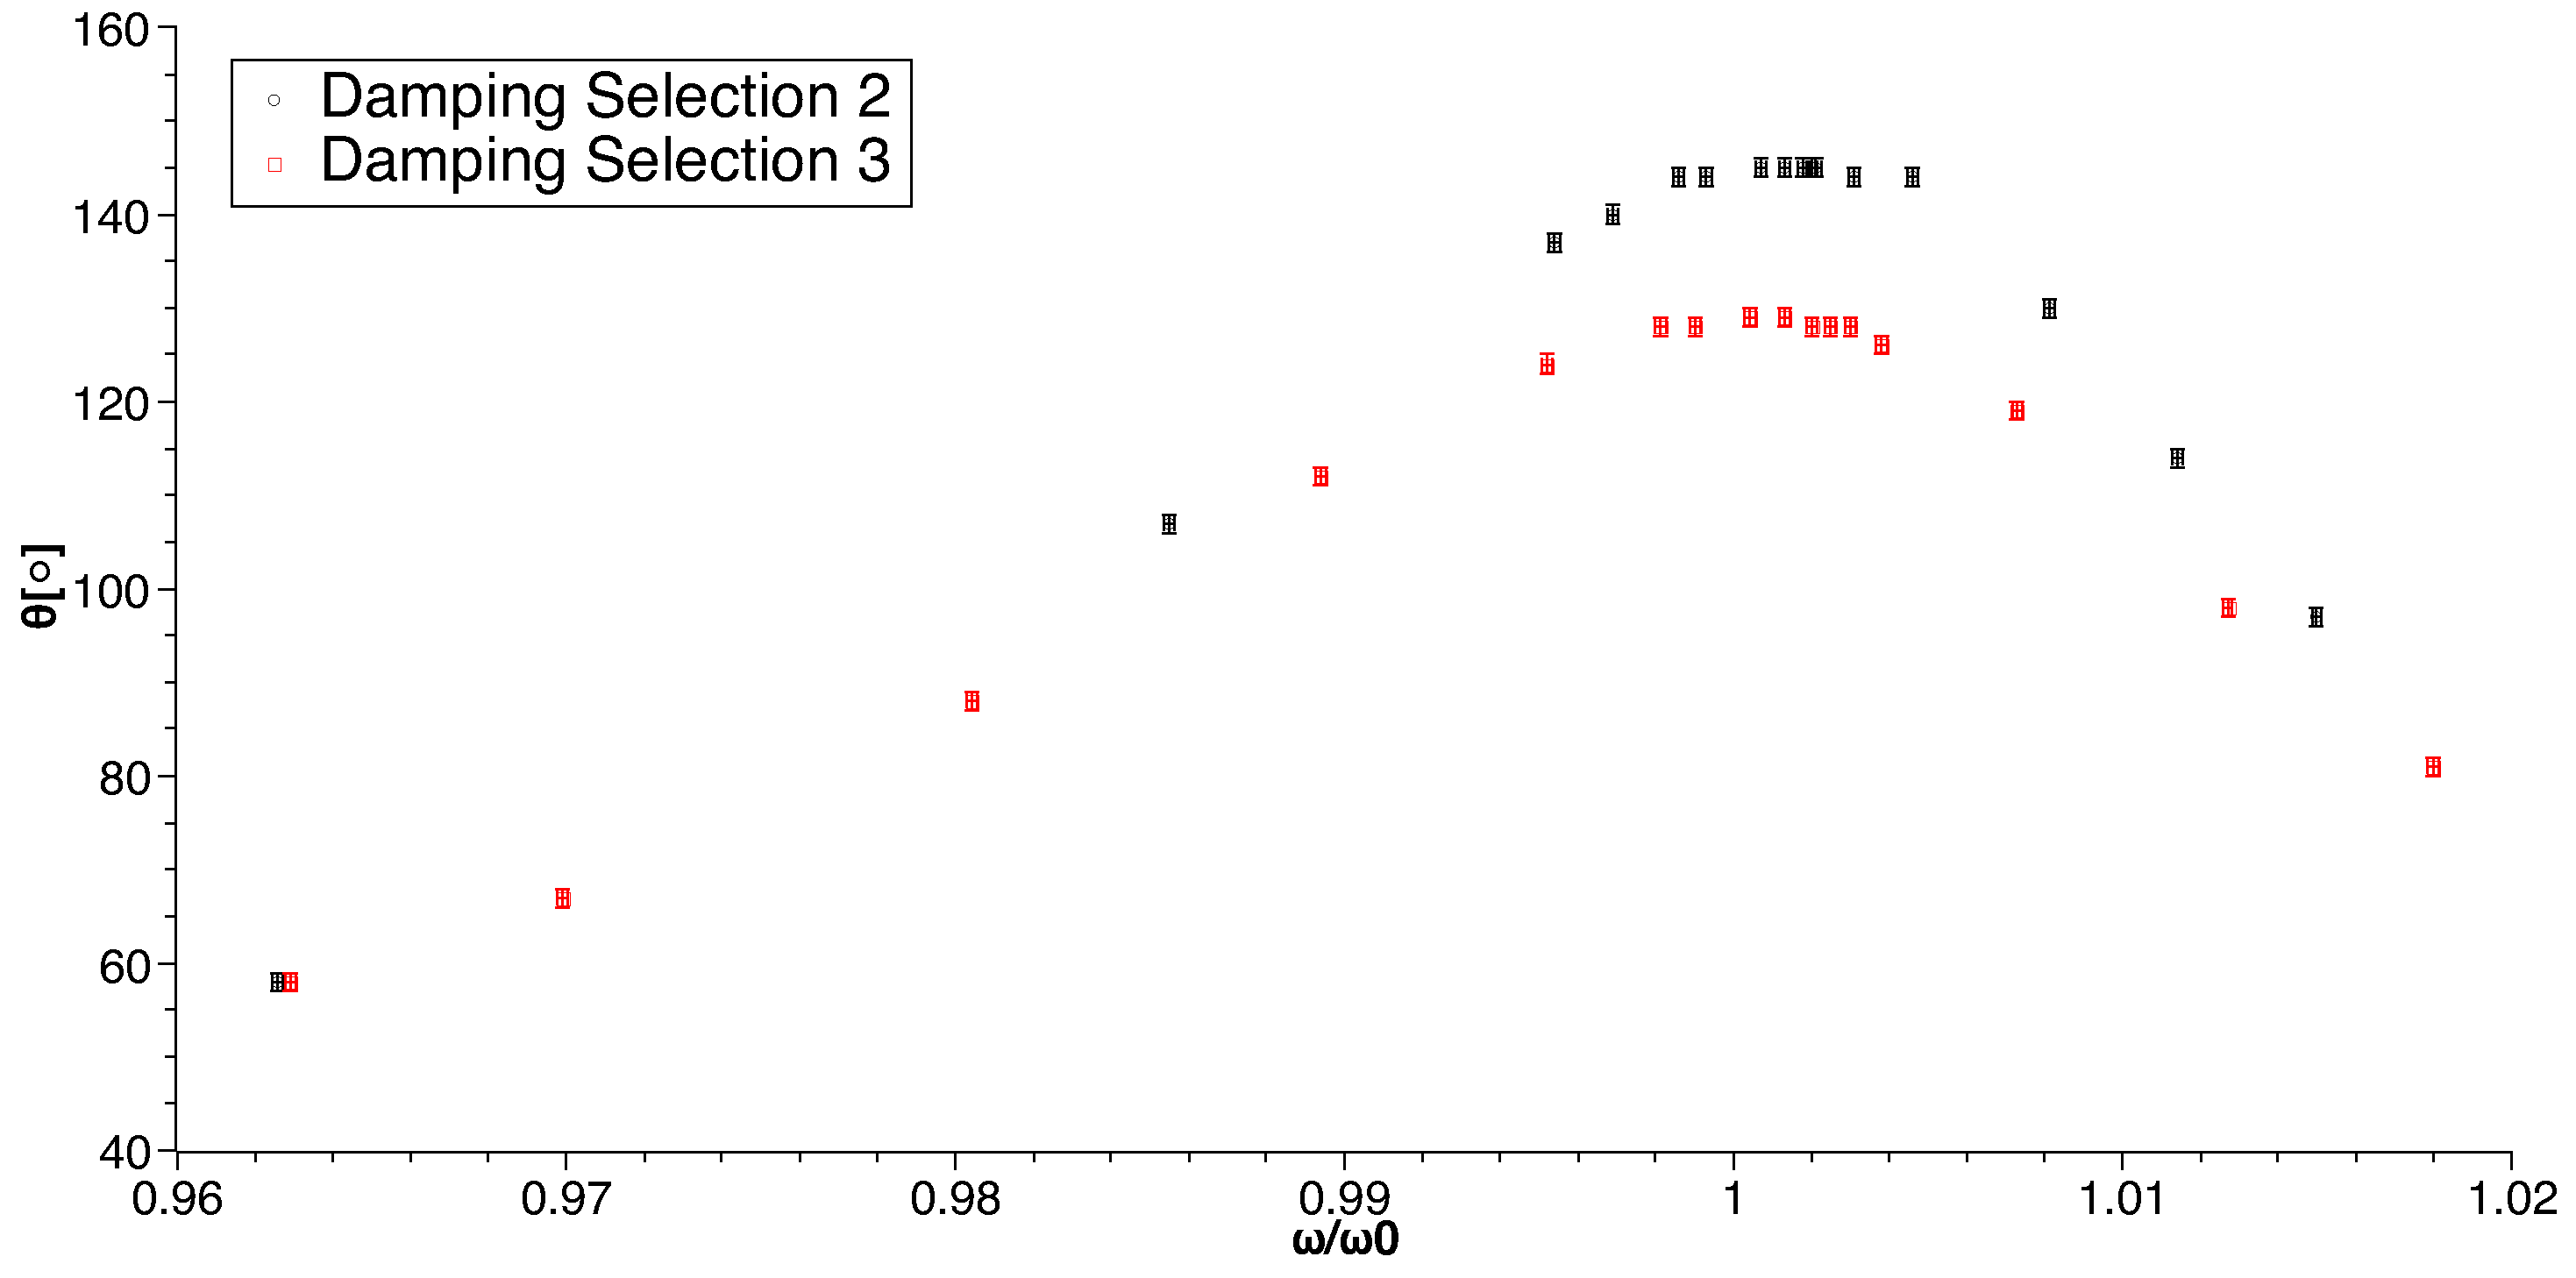
\includegraphics[width=0.96\textwidth]{Figx1_1} 
    \caption{Characteristics of $\theta_{st}-\omega$} 
\end{figure}

\begin{figure}[h] 
    \centering
    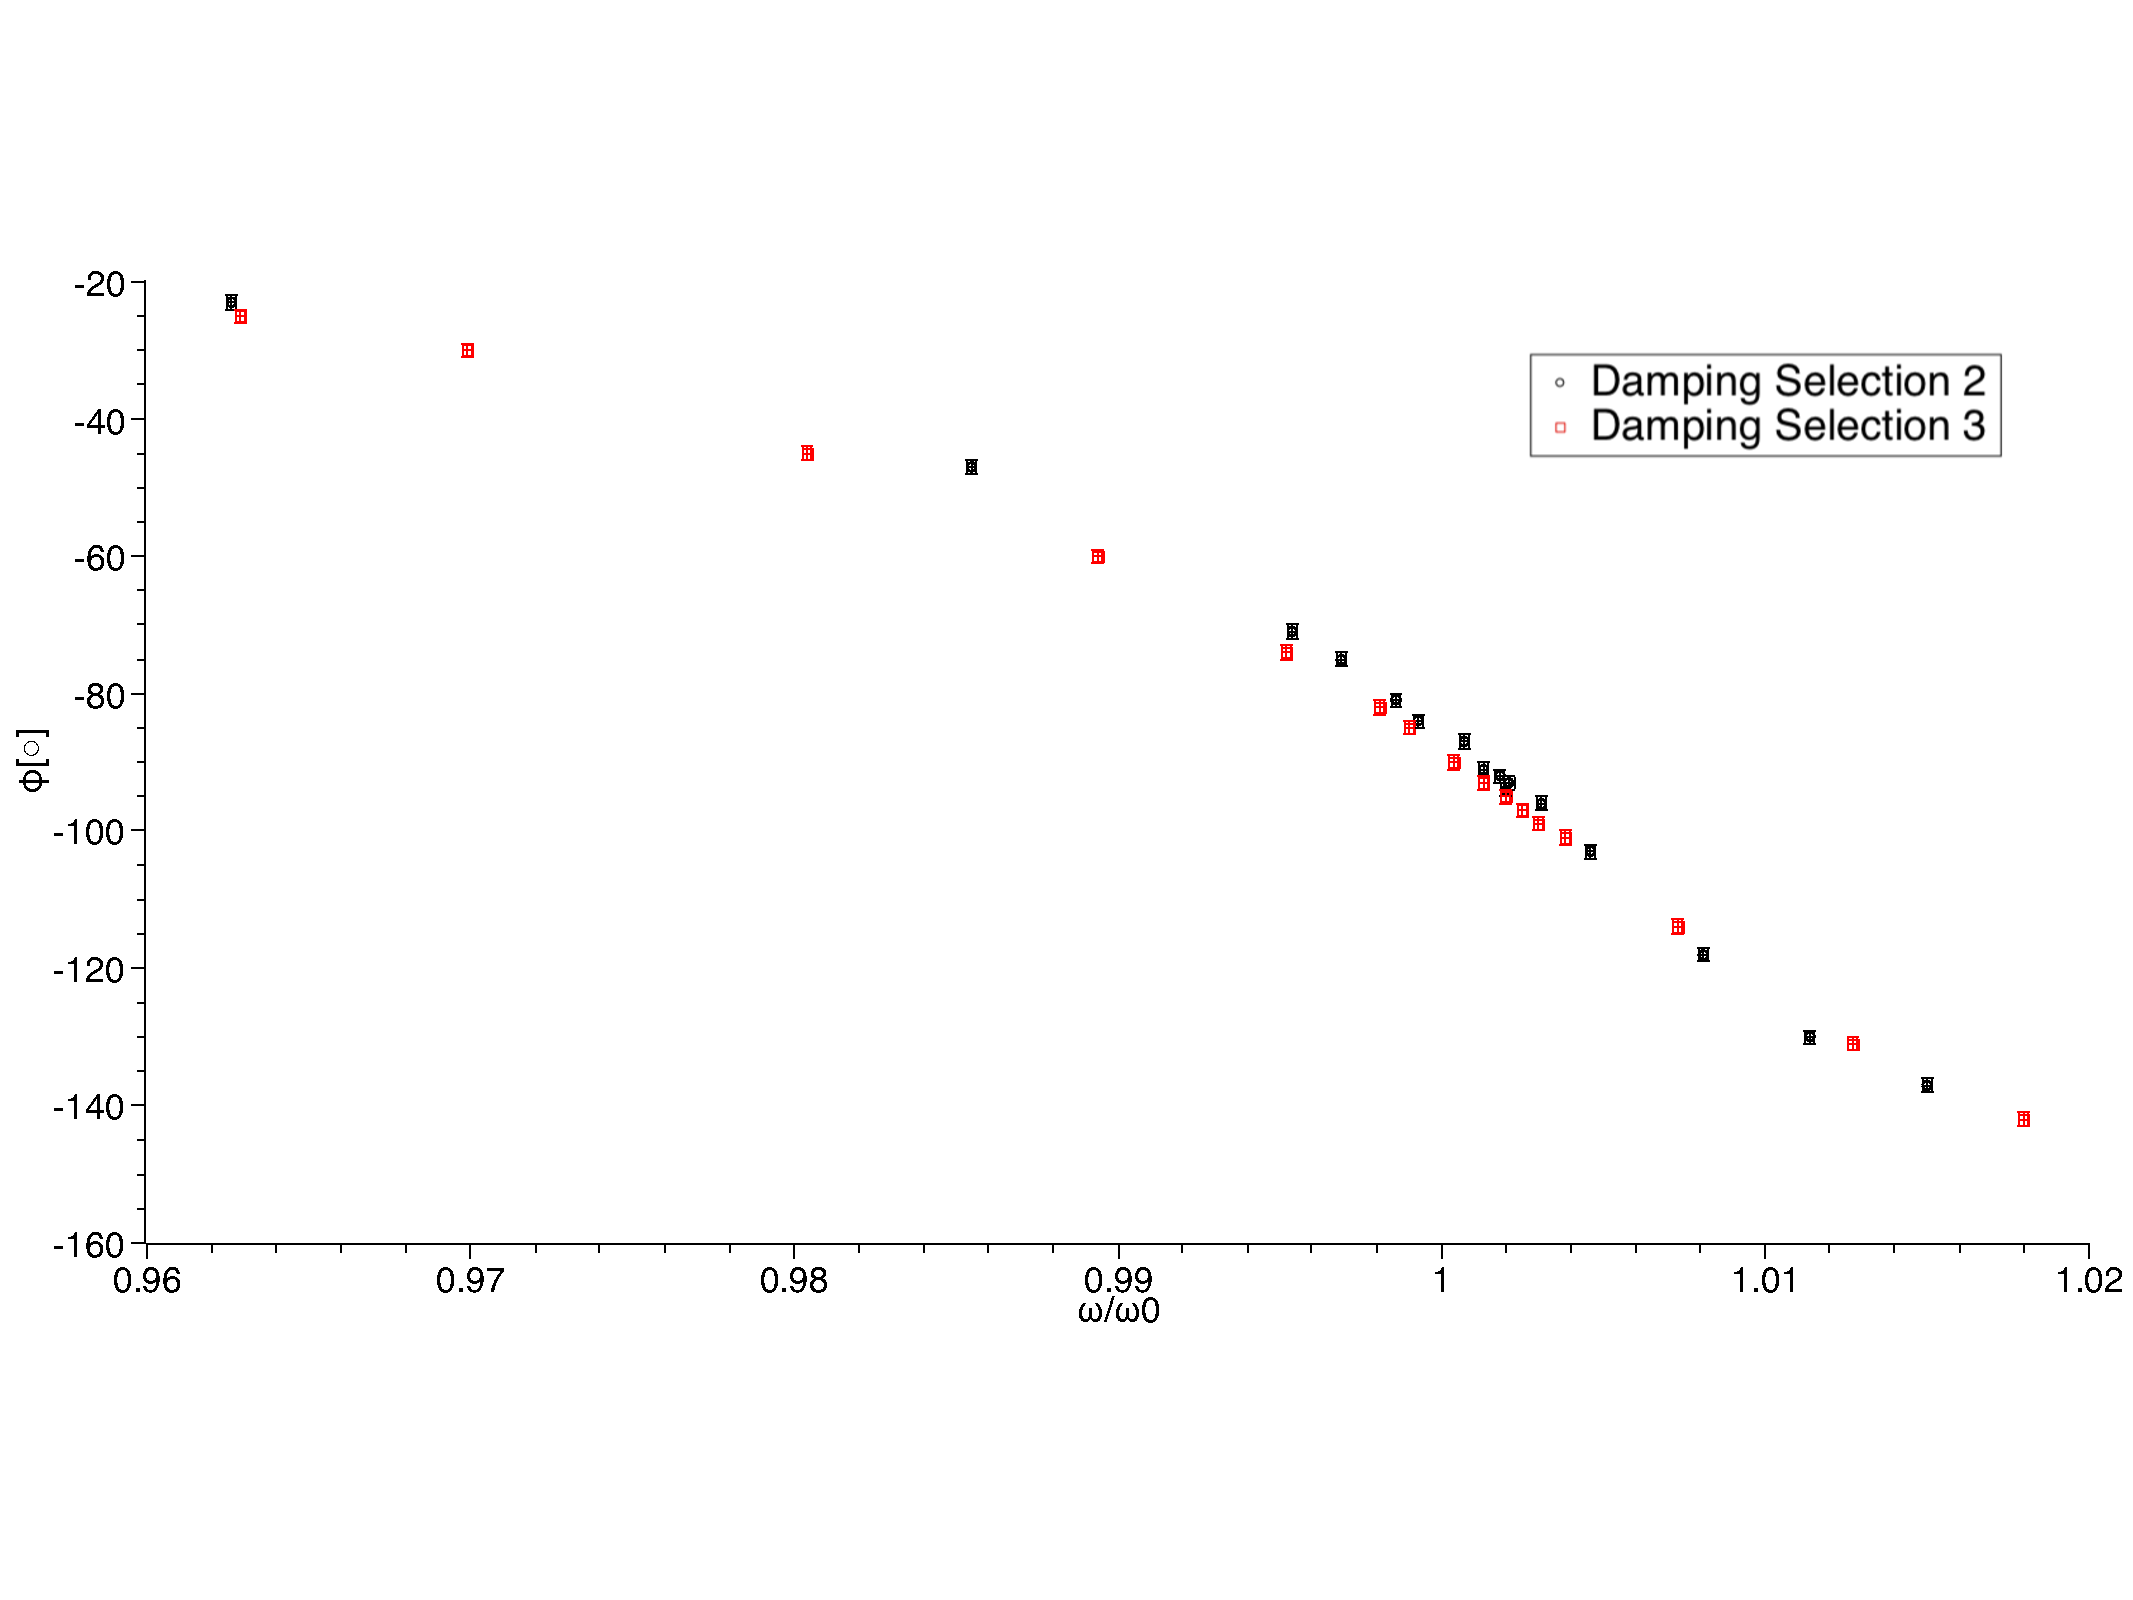
\includegraphics[width=0.96\textwidth]{Figx2_3} 
    \caption{Characteristics of $\varphi-\omega~$} 
\end{figure}

\newpage

\begin{table}[h]
\begin{center}
\begin{tabular}{|c|c|c|c|c|c|}
\hline
\multicolumn{6}{|c|}{ Damping Selection: 2} \\
\hline
   & $10T [s] \pm 0.001 [s]$ & $\varphi[^\circ] \pm 1 [^\circ]$ & $\theta[^\circ] \pm 1 [^\circ]$ & $\omega/\omega_0$ & $u_{\omega/\omega_0}$\\
\hline
1 & 16.426 & 23 & 58 & 0.9626 & 1.4$\times 10^{-4}$\\
2 & 16.044 & 47 & 107 & 0.9855 & 1.4$\times 10^{-4}$\\
3 & 15.884 & 71 & 137 & 0.9954 & 1.4$\times 10^{-4}$\\
4 & 15.860 & 75 & 140 & 0.9969 & 1.4$\times 10^{-4}$\\
5 & 15.833 & 81 & 144 & 0.9986 & 1.4$\times 10^{-4}$\\
6 & 15.822 & 84 & 144 & 0.9993 & 1.4$\times 10^{-4}$\\
7 & 15.800 & 87 & 145 & 1.0007 & 1.4$\times 10^{-4}$\\
8 & 15.790 & 91 & 145 & 1.0013 & 1.4$\times 10^{-4}$\\
9 & 15.783 & 92 & 145 & 1.0018 & 1.4$\times 10^{-4}$\\
10 & 15.778 & 93 & 145 & 1.0021 & 1.4$\times 10^{-4}$\\
11 & 15.780 & 94 & 145 & 1.0020 & 1.4$\times 10^{-4}$\\
12 & 15.762 & 96 & 144 & 1.0031 & 1.4$\times 10^{-4}$\\
13 & 15.739 & 103 & 144 & 1.0046 & 1.4$\times 10^{-4}$\\
14 & 15.684 & 118 & 130 & 1.0081 & 1.4$\times 10^{-4}$\\
15 & 15.633 & 130 & 114 & 1.0114 & 1.4$\times 10^{-4}$\\
16 & 15.577 & 137 & 97 & 1.0150 & 1.4$\times 10^{-4}$\\
\hline
\end{tabular}
\caption{Data table for $\theta_{st}-\omega$ and $\varphi-\omega$ characteristics}
\end{center}
\end{table}

\newpage

\begin{table}[h]
\begin{center}
\begin{tabular}{|c|c|c|c|c|c|}
\hline
\multicolumn{6}{|c|}{ Damping Selection: 3} \\
\hline
   & $10T [s] \pm 0.001 [s]$ & $\varphi[^\circ] \pm 1 [^\circ]$ & $\theta[^\circ] \pm 1 [^\circ]$ & $\omega/\omega_0$ & $u_{\omega/\omega_0}$\\
\hline
1 & 16.420 & 25 & 58 & 0.9629 & 1.4$\times 10^{-4}$\\
2 & 16.301 & 30 & 67 & 0.9699 & 1.4$\times 10^{-4}$\\
3 & 16.126 & 45 & 88 & 0.9804 & 1.4$\times 10^{-4}$\\
4 & 15.981 & 60 & 112 & 0.9894 & 1.4$\times 10^{-4}$\\
5 & 15.888 & 74 & 124 & 0.9952 & 1.4$\times 10^{-4}$\\
6 & 15.841 & 82 & 128 & 0.9981 & 1.4$\times 10^{-4}$\\
7 & 15.827 & 85 & 128 & 0.9990 & 1.4$\times 10^{-4}$\\
8 & 15.804 & 90 & 129 & 1.0004 & 1.4$\times 10^{-4}$\\
9 & 15.790 & 93 & 129 & 1.0013 & 1.4$\times 10^{-4}$\\
10 & 15.780 & 95 & 128 & 1.0020 & 1.4$\times 10^{-4}$\\
11 & 15.772 & 97 & 128 & 1.0025 & 1.4$\times 10^{-4}$\\
12 & 15.764 & 99 & 128 & 1.0030 & 1.4$\times 10^{-4}$\\
13 & 15.751 & 101 & 126 & 1.0038 & 1.4$\times 10^{-4}$\\
14 & 15.697 & 114 & 119 & 1.0073 & 1.4$\times 10^{-4}$\\
15 & 15.612 & 131 & 98 & 1.0127 & 1.4$\times 10^{-4}$\\
16 & 15.531 & 142 & 81 & 1.0180 & 1.4$\times 10^{-4}$\\
\hline
\end{tabular}
\caption{Data table for $\theta_{st}-\omega$ and $\varphi-\omega$ characteristics}
\end{center}
\end{table}



%----------------------------------------------------------------------------------------
%	SECTION 5
%----------------------------------------------------------------------------------------
\newpage

\section{\textsc{Conclusion and Discussion}}
The experiment is divided into three parts. In the first part, we measured the natural frequency of the balance wheel. By turning the "Period Selection" to "10", we measured the 10 periods of the oscillation. After repeating four times, we finally obtained 4 data. Then we use the formula to calculate out our natural frequency: 
\begin{center}
$\displaystyle \omega_0 = \frac{2\pi}{T} = \frac{2\pi}{\overline{10T}/10}$
\end{center}
Then we got our natural frequency as $\displaystyle \omega_0 = 3.9739 [s^{-1}] \pm 0.0004[s^{-1}]$, with a relative uncertainty $0.01\%$. 
\par Generally speaking, the uncertainty is satisfactory for us. However, we still do some improvements about it: Although the certainty is not large, we will use the natural frequency throughout the experiment. Hence even a minor improvement will be beneficial to our overall precision of experiment later. Since the uncertainty mainly comes from Type A and Type B, and the Type A uncertainty occurs due to the limitations of the apparatuses, we can try our best to decrease the Type B uncertainty. In our experiment, we measured 4 data for the period. If we are able to collect more data. For example, we repeat the experiment for 10 times, then chances are that our uncertainty of natural frequency become lower. 
\par In the next part, we measured the damping coefficient. We recorded the changing amplitudes successively, and then find out the damping coefficient through the following formula:
\begin{center}
$\displaystyle \beta = \frac{1}{5T}ln\frac{\theta_i}{\theta_{i+5}}$
\end{center}
Then we obtained our results: $\displaystyle \beta = 0.056 [s^{-1}] \pm 0.004[s^{-1}]$, with a relative uncertainty about $7\%$.
\par In this experiment, we have a relative large deviation compared with the previous errors. The reasons are complicated. From one aspect, the measurements becomes more complex, which makes the uncertainty more likely to increase. From another aspect, In this process, since we should set the balance wheel at 150 degrees at rest before letting it rotate, the uncertainty may comes from our misplacing of the wheel. In other words, it hard for us to place the wheel at accurate 150 degrees simply by eyes. Hence large uncertainty may occur here. Moreover, if we take into consideration the influence of air drag or the instability of the resonator, the uncertainty will be even larger. 
\par To minimize our uncertainty, we can first release the balance in the exact angle of 150 degrees with the help of the angular ruler. Also, we can try to do the experiment in the place where the wind is relatively gentle, so that the disturbance will be less, and our results will become more accurate
\par Finally, in the last part, we focused on the situation where a periodically changing external force is added to our system. According to our deduction in Introduction part, the relationship between $\theta_{st}/\varphi$ and $\omega$ should be as follows:
\begin{center}
$\displaystyle \theta_{st} = \frac{\mu}{\sqrt{(\omega_0^2 - \omega^2)^2 + 4\beta^2\omega^2}} $ \\[3 mm]
$\displaystyle \varphi = arctan(\frac{2\beta \omega}{\omega^2-\omega_0^2})$
\end{center}
\par Since in this experiment, the uncertainty can't be easily analysed numerically, we plot the theoretical curve for our experiment. With the help of Matlab, the theoretical plot for $\theta_{st}$ vs. $\omega$ are shown as follows (Fig.6 and Fig.7):
\begin{figure}[h] 
    \centering
    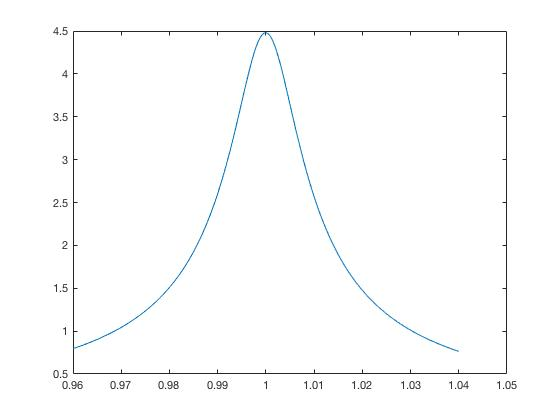
\includegraphics[width=0.6\textwidth]{Figc1} 
    \caption{Theoretical characteristics of $\theta_{st}-\omega$} 
\end{figure}
\begin{figure}[h] 
    \centering
    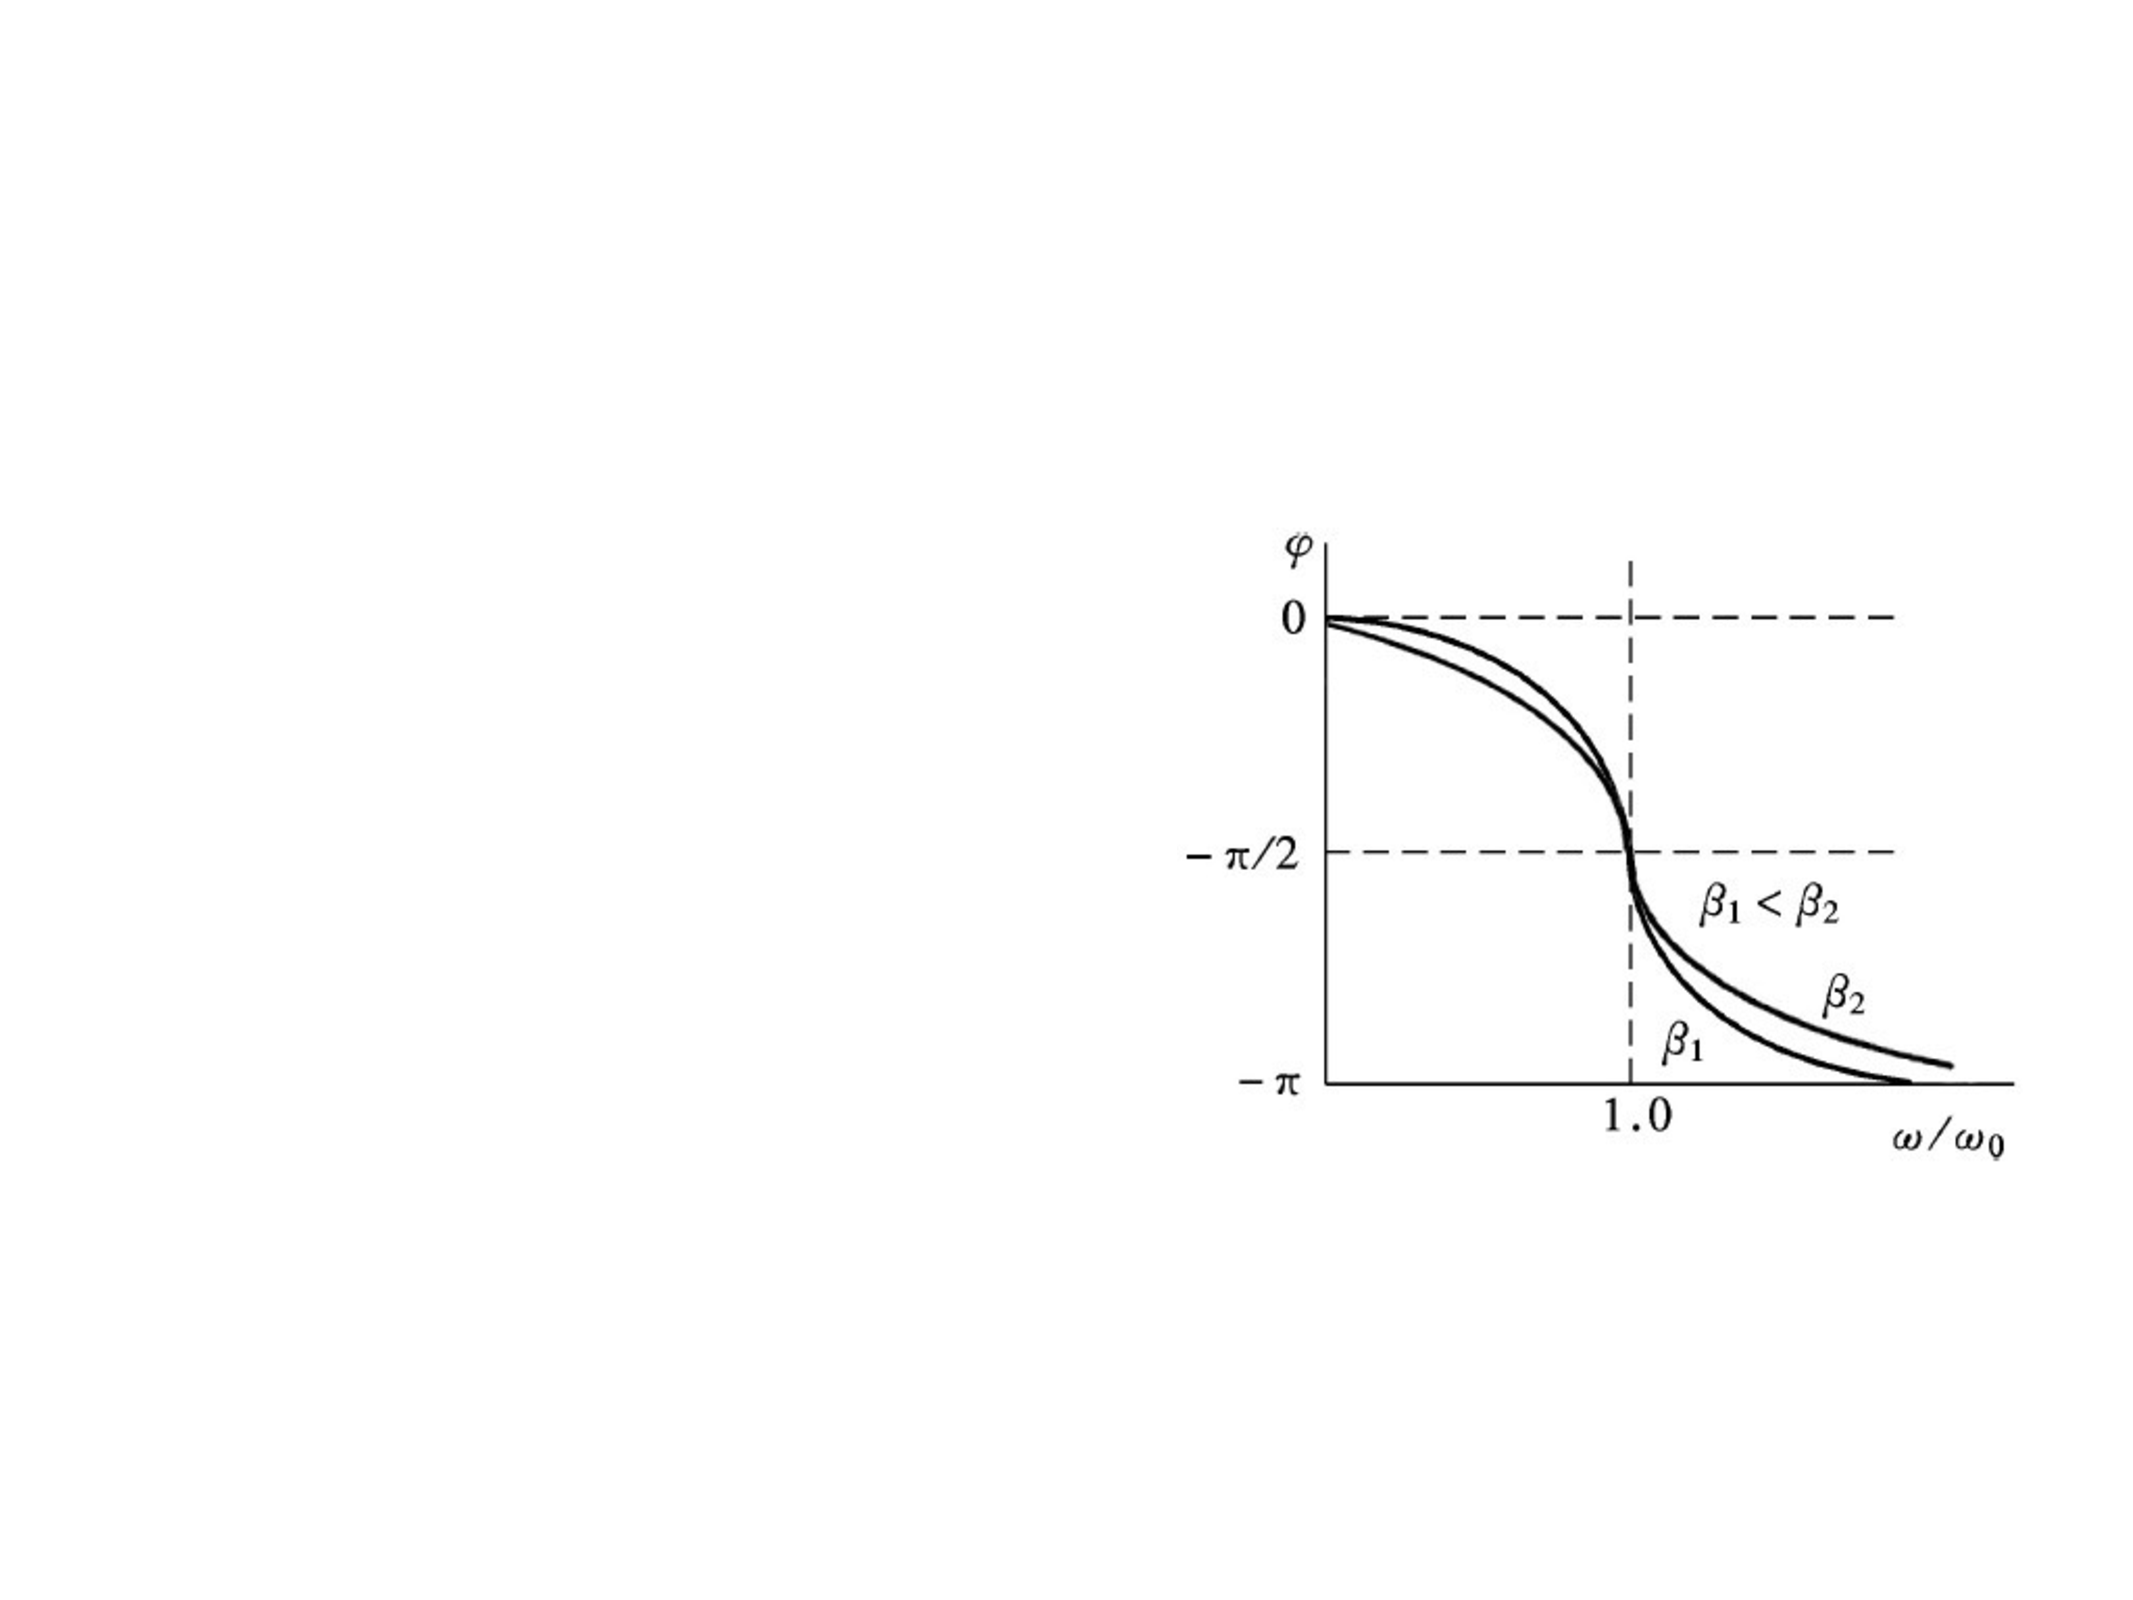
\includegraphics[width=0.6\textwidth]{Figc2} 
    \caption{Theoretical characteristics of $\varphi-\omega$ \cite{labmanual}} 
\end{figure}
\newpage
\par From the comparison of our experimental plot and theoretical plot, we find out that there exists some uncertainties. 
\par One significant difference is that our plot is not as smooth as the theoretical plot, which may be caused by the instability of our reading. To be more specific, we may not wait enough time before the system becomes completely steady. As a result, the data we collected may be those who are not at equilibrium, leading to the not-smooth curve. Besides, our curve tends to be a little bit "steep" compared with the theoretical one. This may comes from the existence of air drag, which makes the curve an irreversible deformation. 
\par To minimize these issues, first, we can be patient while doing our experiment. We should wait a few seconds so that we make sure our balance wheel has reaches its equilibrium state. After that, the data collected can be accurate. Besides, in the process we begin to measure its period, during which the amplitude begins to change, it means we are not at the equilibrium. Hence in this case we should measure the period again. 
\par Moreover, in terms of air drag, we can do this experiment at a wind-gentle environment with windows closed, and during the process of experiment, we shouldn't move or disturb the resonator. In this way the external disturbance can be made as less as possible, which results in the decrease of error.
\par Lastly, in our lab, there is another place which we can improve, i.e., when collecting the data, it's better for us to collect more data when $\omega/\omega_0$ is approaching 1, because at this time the curve tends to decrease largely. Thus more data points can indicate a more accurate result. Besides, when collecting the data, we 'd better control our phase lag so that $\varphi$ is symmetric about the line $\omega/\omega_0 = 1$ so that we can better find out the general trend. To be more specific, in our data, if we could collect a data point where $\varphi \approx 160^\circ$, our plot will be symmetric and closer to the theoretical one.

%----------------------------------------------------------------------------------------
%	SECTION 6
%----------------------------------------------------------------------------------------

\begin{appendices} 
      \section{\textsc{Measurement uncertainty analysis}} 
      See the Worksheet.
      \section{\textsc{Data sheet}} 
      See the attached data sheet.
  \end{appendices} 

%----------------------------------------------------------------------------------------
%	BIBLIOGRAPHY
%----------------------------------------------------------------------------------------

\begin{thebibliography}{9}
\bibitem{labmanual} Krzyzosiak, M. \& VP141 TA Groups.
\textit{Exercise 5 - lab manual [rev 4.3].pdf}. 
2019.
\end{thebibliography}


%----------------------------------------------------------------------------------------


\end{document}
